\documentclass{standalone}
\usepackage{plotstyle}

\begin{document}

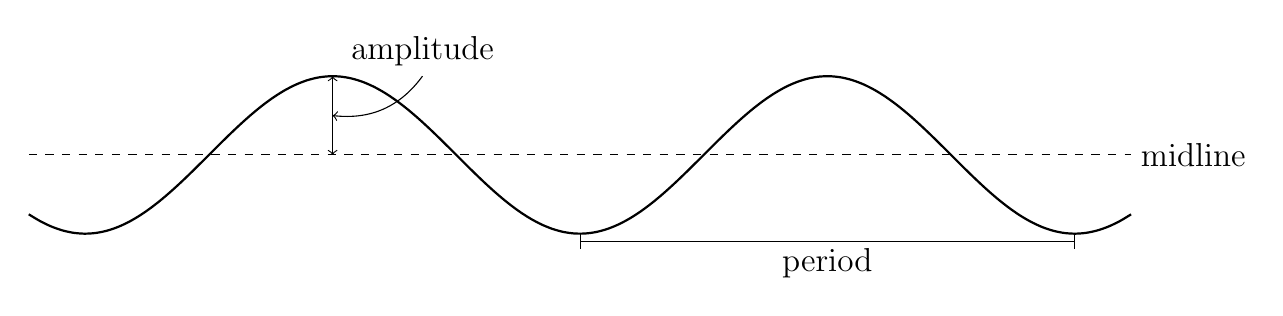
\begin{tikzpicture}[font=\large]
    % Set up styles for labeling
    \tikzstyle{brace} = [decorate,decoration={brace,amplitude=10pt,mirror},yshift=-5pt]
    \tikzstyle{arrow} = [->,thick]

    % Draw the sinusoidal graph
    \draw[thick, domain=-7:7, samples=100, smooth] plot
        ({\x}, {-cos(\x r)});

    % Draw the midline
    \draw[dashed] (-7,0) -- (7,0);

    % Label the amplitude
    \draw[<->] (-pi,0) -- (-pi,1) node[midway, left] {};
    \draw[->] (-2,1) node[above] {amplitude} to[bend left] (-pi,0.5);
     
    % Label the period
    \draw[|-|] (0,-1.1) -- (2*pi,-1.1)
        node[midway, yshift=-8pt] {period};

    % Label the midline
    \node at (7, 0) [right] {midline};

\end{tikzpicture}

\end{document}